\begin{figure*}[h!]
    \centering
    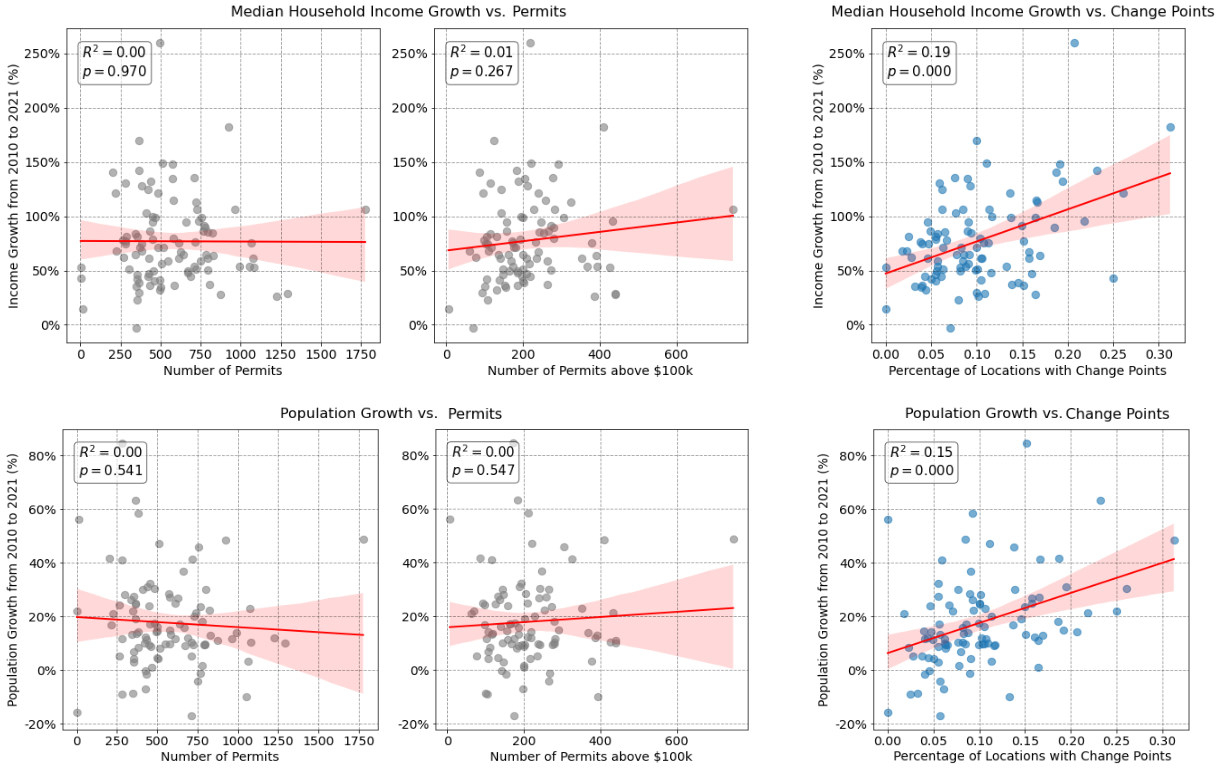
\includegraphics[width=0.93\linewidth]{figure/acs.png}
    \caption{Linear correlation with socio-demographic indicators. \textbf{Top:} Median household income. \textbf{Bottom:} Population size. Each dot represents a Seattle census tract. The change detection results show statistically significant correlations with socio-demographic metrics, in contrast to construction permit data which lacks such correlation.}
    \label{fig:acs}
\end{figure*}

% \begin{figure*}[h!]
%     \centering
%     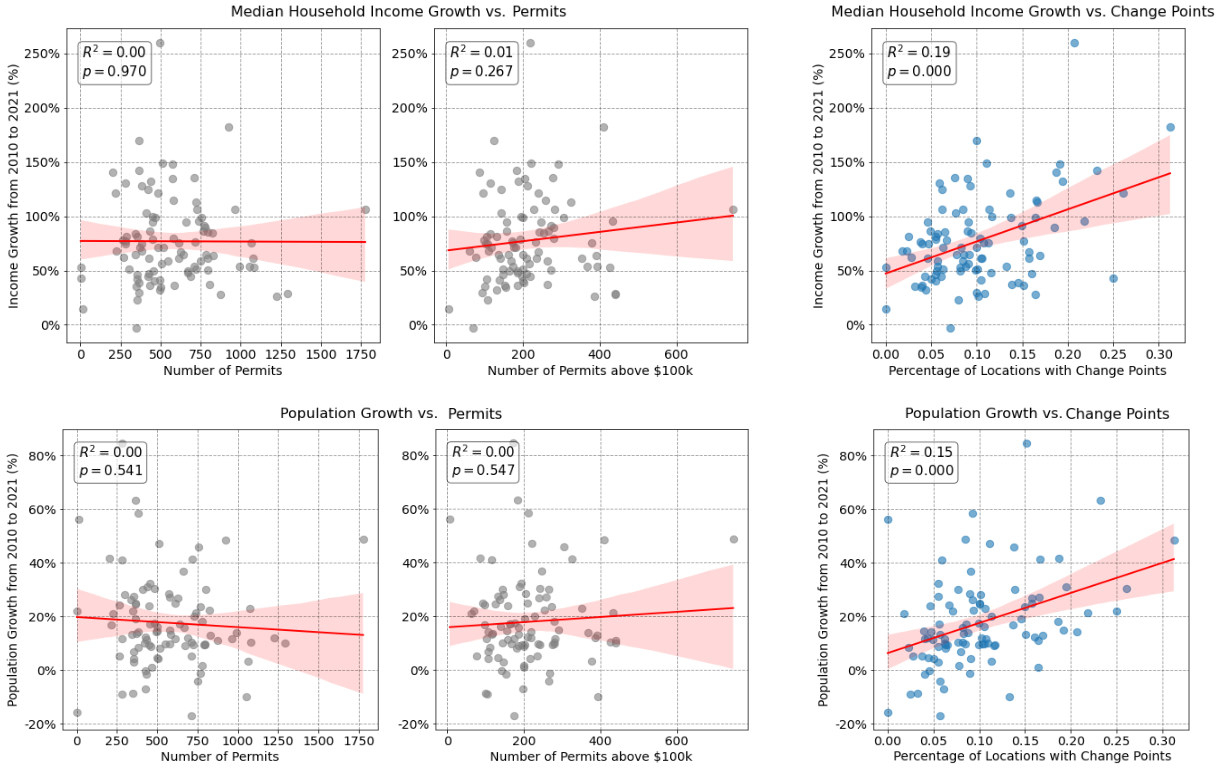
\includegraphics[width=0.9\linewidth]{figure/acs.png}
%     \caption{Correlation of change detection results with socio-demographic indicators. \textbf{Top:} Median household income. \textbf{Bottom:} Population size. Each dot corresponds to a Seattle census tract. Notably, these results exhibit significant correlations with socio-demographic metrics, unlike the construction permit data.}
%     \label{fig:acs}
% \end{figure*}


% \begin{figure*}[h!]
%     \centering
%     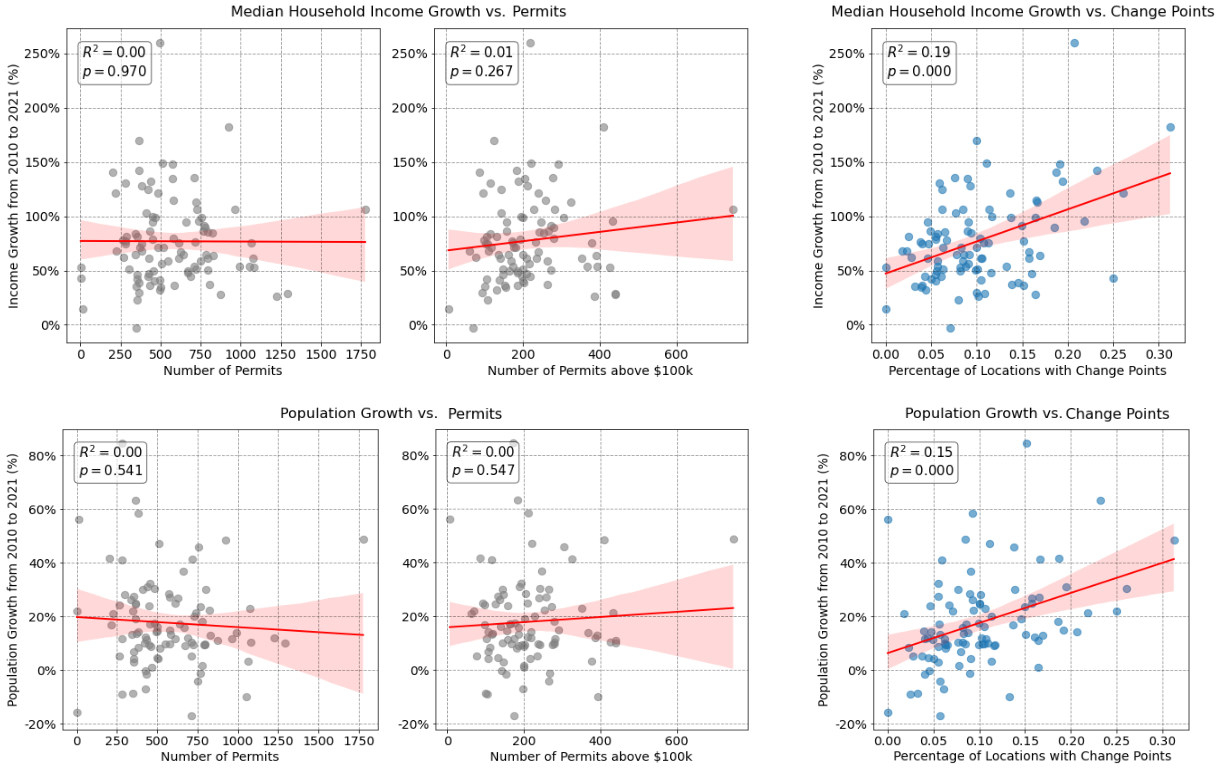
\includegraphics[width=0.96\linewidth]{./figure/acs.png}
%     \caption{Linear correlation with social-demographic data. \textbf{Top:} Median household income. \textbf{Bottom: } Population size. Each dot represents a census tract in Seattle. Change detection results demonstrates statiscally signifcant correlations with social-demographic data, while construction permit data fail to do so.
%     }
%     % between ACS attributes and total number of predicted change points in each census tract vs. correlation between ACS attributes and total number of construction permits in each census tract}
%     \label{fig:acs}
% \end{figure*}